\section{Verplank diagram}
\label{Verplank_diagram}
When initially designing Fingerdrums a Verplank diagram was created to help specify and explain the idea further, see \autoref{fig:Verplank} . 
\blankline

\begin{figure}[H]
\centering
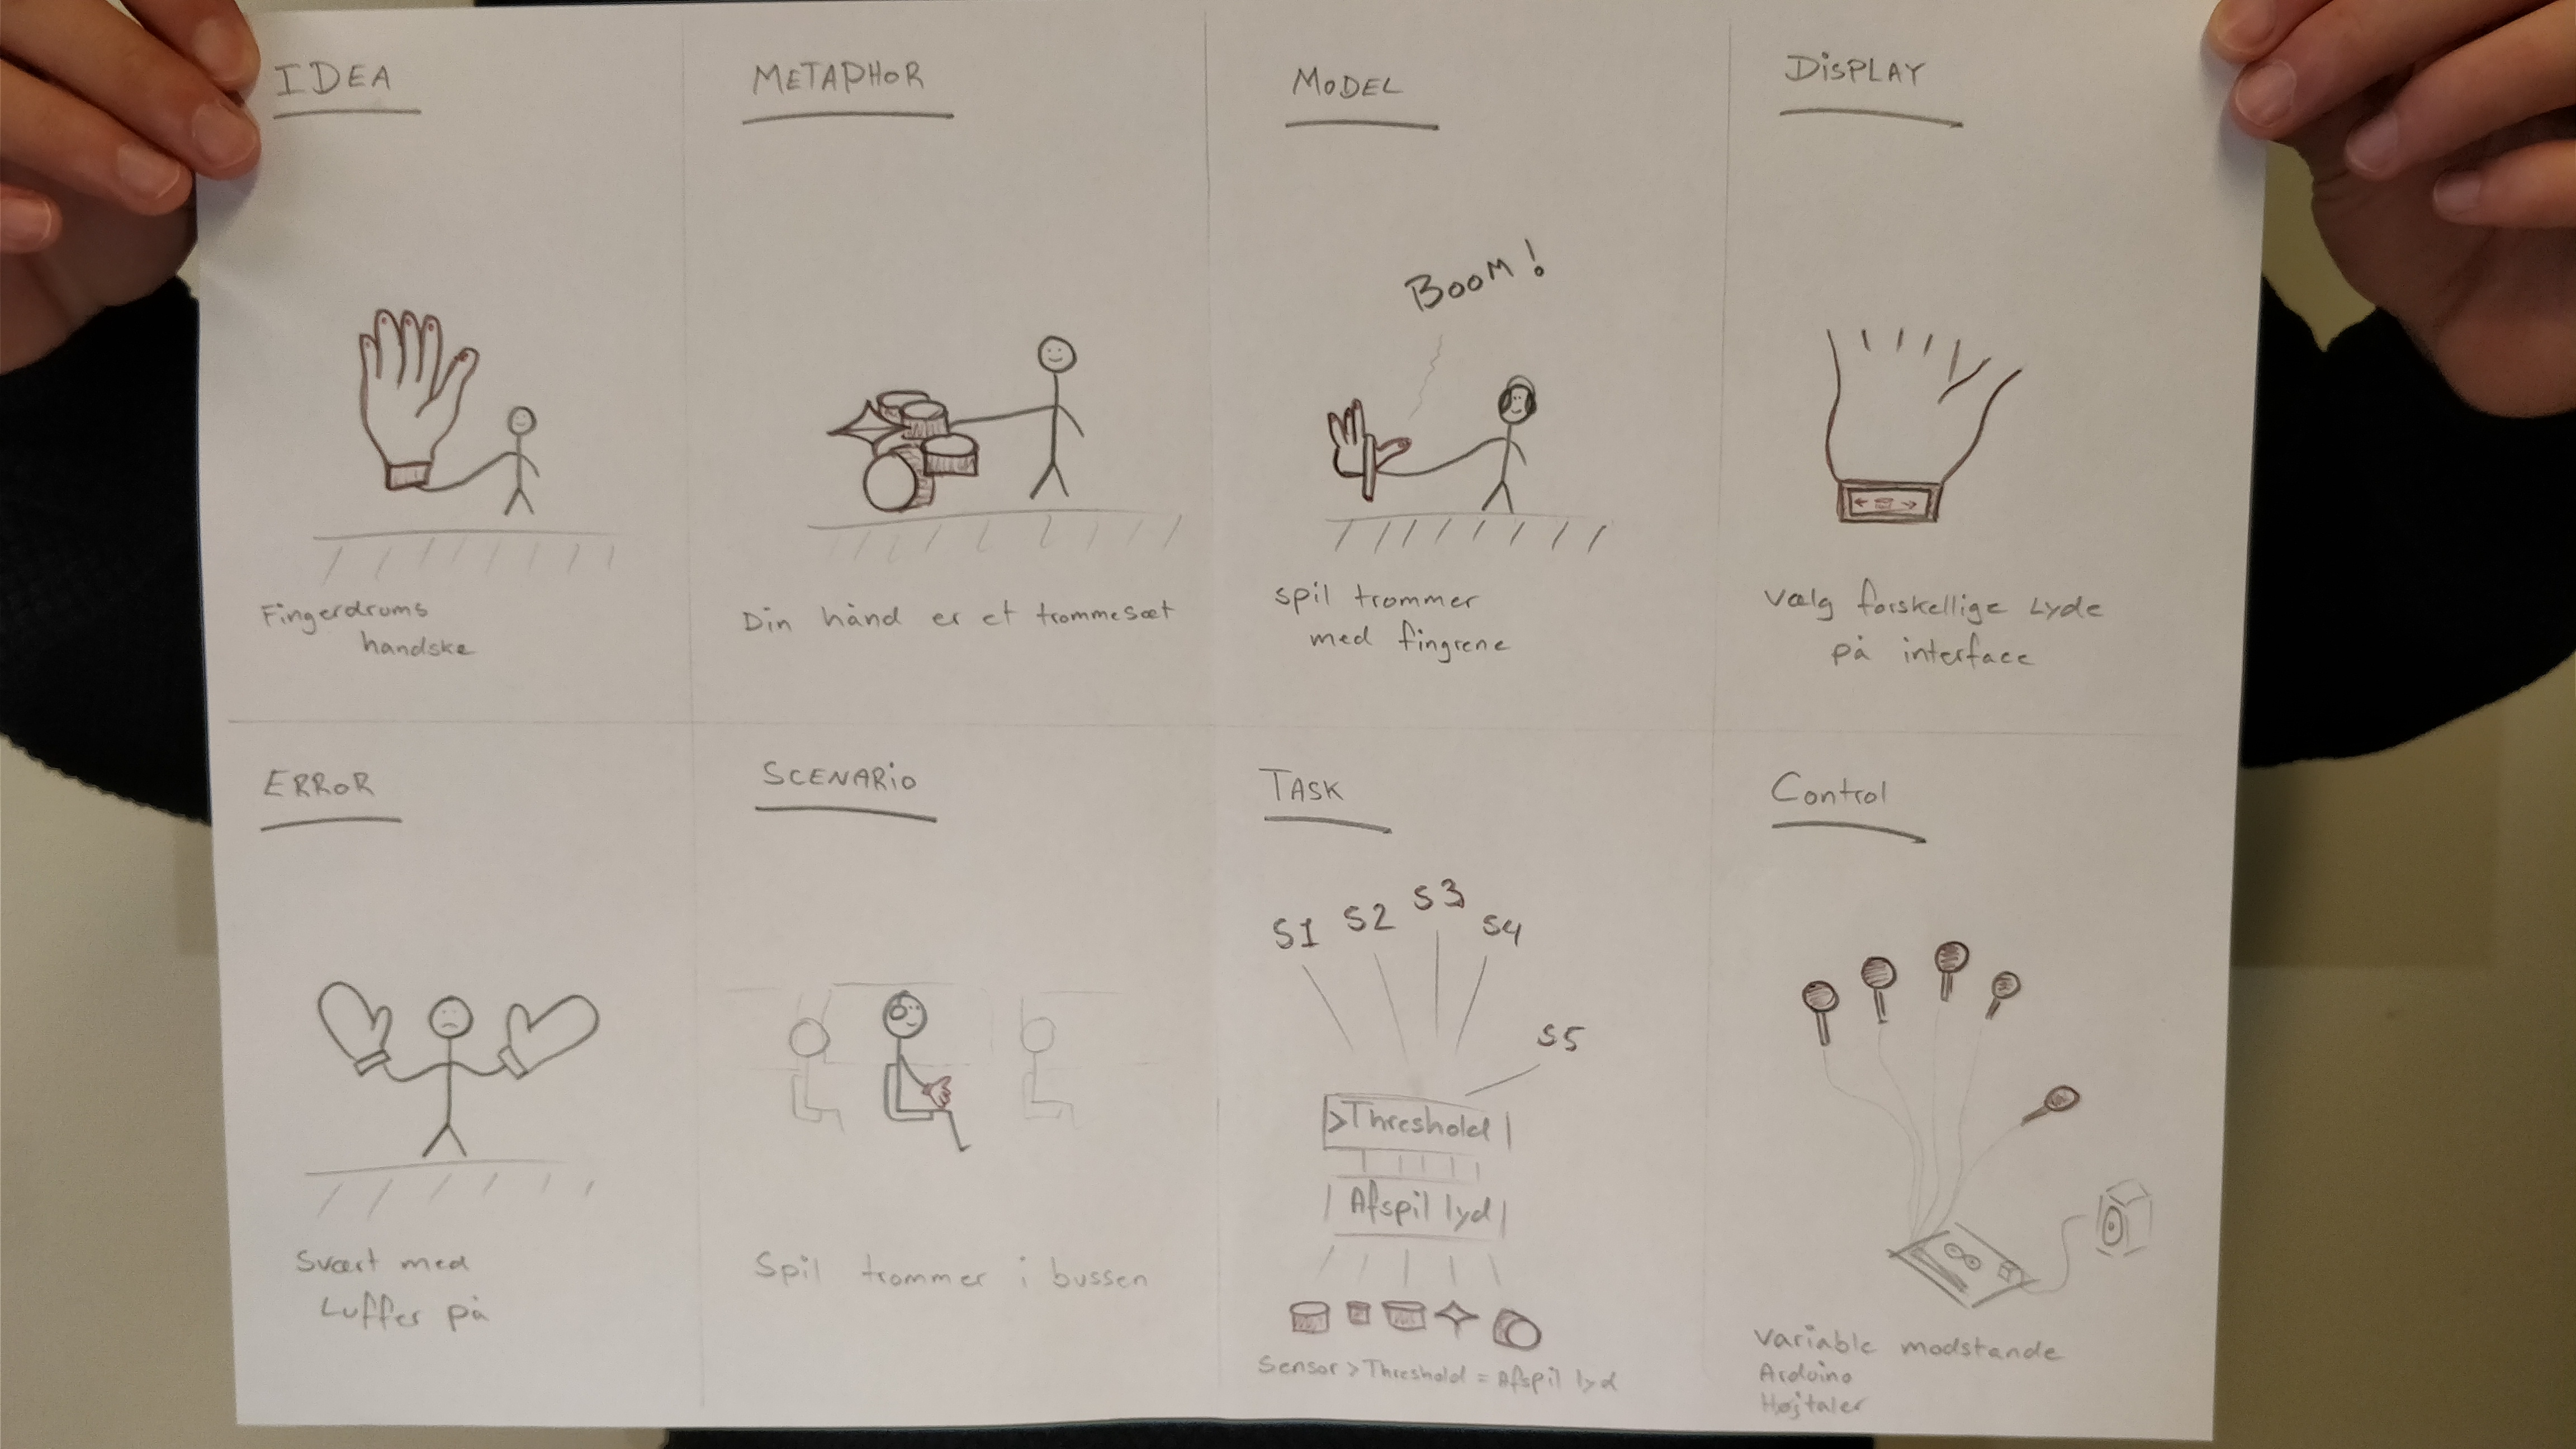
\includegraphics[scale = 0.1]{Figure/Billeder/IMG_20171114_121155.jpg}
\caption{Verplank diagram for the Fingerdrums prototype.}
\label{fig:Verplank}
\end{figure}

\textbf{Idea}\\
A glove that alows you to play the drums on any surface.
\blankline

\textbf{Metaphore}\\
Your hand is the drum set.  
\blankline

\textbf{Model}\\
Play the drums with you fingers without an actual drum set.
\blankline

\textbf{Display}\\
Small display on the wrist which shows the type of drum sounds are currently being used.
\blankline

\textbf{Error}\\
The touchscreen on your phone will not be usable when waring the glove. Drumming on any object will still produce a sound, which could be disruptive, depending on the object. Can't be used when wearing mittens.
\blankline

\textbf{Scenario}\\
You can play th drums on the bus on the way home from work without having to bring a actual drum set.
\blankline

\textbf{Tasks}\\
Check if any finger is being pushed over the threshold, if they are, play a sound.
\blankline

\textbf{Control}\\
Variable resistors sending signal through micro controller and out through a speaker.